\documentclass[12pt]{article}

\usepackage{sbc-template}

\usepackage{graphicx,url}

%\usepackage[brazil]{babel}   
\usepackage[latin1]{inputenc}  

     
\sloppy

\title{PRECISAMOS COLOCAR UM TÍTULO AINDA}

\author{Lucas Takeshi R. Palma\inst{1}, Márcio Sakamoto Shibao\inst{1}}


\address{Caelum - Ensino e Inovação\\
  CEP 04101-300 -- São Paulo -- SP -- Brasil
  \email{\{lucas.takeshi,marcio.shibao\}@caelum.com.br}
}

\begin{document} 

\maketitle

\begin{abstract}
  
\end{abstract}
     
\begin{resumo} 
Em métodos ágeis, convivemos com diversos problemas na nossa forma de trabalhar. Uma das formas de enfrentá-los é através da retrospectiva, cujo objetivo é promover o princípio da melhoria contínua no time, seja na qualidade do produto ou na forma de trabalhar. Mas com o aumento da globalização surgiram novos formatos de equipes, como os times distribuídos, e novos desafios para realizar esta reunião. Este artigo mostra a construção de uma pesquisa sobre como os times fazem para promover melhoria contínua nos dias de hoje e uma análise sobre os dados obtidos. 
\end{resumo}

\section{Indrodução}

O conceito sobre o que é a agilidade surgiu a partir do Manifesto Ágil \cite{manifesto:01}. Os seus quatro valores e doze princípios são essenciais para que todo time que quer ser ágil, já que incentivam essas equipes a melhorar a qualidade do trabalho executado e atender às expectativas dos clientes, ainda que essas sofram constantes mudanças. Apesar de cada princípio ter a sua importância, aquele que estimula o time a estar em constante evolução em todos os aspectos é a melhoria contínua:

\begin{quote}
  \textit{``At regular intervals, the team reflects on how to become more effective, then tunes and adjusts its behavior accordingly.''}\cite{manifesto:01}
\end{quote}

Diversos estudos na comunidade abordam como promover a melhoria contínua. Um bom exemplo é o Lean, a filosofia por trás do modelo de produção da Toyota \cite{ohno:88}. Ela apresenta o conceito do Kaizen, que defende que todas as pessoas, independente da sua posição na empresa, são responsáveis por pensar e agir para melhorar continuamente o processo e o produto da companhia.

Nos métodos ágeis, a prática que mais se destaca atualmente é a retrospectiva. Segundo Derby e Larsen \cite{retrospectives:06}, a retrospectiva é uma reunião especial em que o time se junta para investigar e melhorar seus métodos - um tempo dedicado à aprendizagem, que funciona como um catalisador de mudanças e ações. Diferente das tradicionais lições aprendidas, esta prática foca tanto no processo de desenvolvimento, quanto nas questões humanas do projeto.

\section{Desafios da retrospectiva}

Atualmente existem vários livros, artigos e sites com catálogos de diferentes formatos e atividades para esta reunião, como o Fun Retrospectives \cite{fun:14}, Retrospective Handbook \cite{handbook:13} e o Agile Retrospectives \cite{retrospectives:06}. Mesmo com essa grande quantidade de material disponível e o amplo uso da retrospectiva, a sua aplicação pode não apresentar os resultados desejados. Trata-se de um encontro que envolve uma grande discussão entre os integrantes a respeito do processo de desenvolvimento, do projeto e de questões pessoais. Então dependendo do contexto do time, ela pode se tornar uma reunião complexa. Alguns dos problemas conhecidos são:

\begin{enumerate}
  \item Ultrapassar a duração programada para a reunião.
  \item Falta de intimidade entre integrantes para discussões profundas e, algumas vezes, do ambito pessoal.
  \item Reuniões em que as discussões foram superficiais e as ações encontradas foram de pouco valor.
  \item Falta de engajamento dos integrantes em participar da runião por não perceber seu valor ou por algum desgaste que começaram a ter com ela.
  \item Dificuldade para agendar a data para realizar o encontro com todos os integrantes.
\end{enumerate}

Existem estratégias para enfrentar estes desafios, como o uso do facilitador, retrospectiva da retrospectiva no fim da reunião, variação das atividades, entre outros. Mas dada a sua complexidade, novos problemas acabam aparecendo e alguns dos antigos reaparecem mesmo adotando providências.

\subsection{A retrospectiva em um contexto global}

Quando o Manifesto Ágil \cite{manifesto:01} surgiu em 2001, a grande maioria dos times trabalhavam no mesmo lugar. Era difícil encontrar casos de equipes distribuídas em diversas regiões, até por conta da limitação dos recursos na época, como a internet. Então muitas das práticas ágeis, como a retrospectiva,  tiveram como base apenas cenários de times locais.
  
Com o passar do tempo, tanto o mercado quanto a academia mudaram. O aumento da globalização e a evolução da internet fizeram com que diversas empresas investissem vada vez mais em times distribuídos ágeis. Segundo a State of Agile Report \cite{version:12}\cite{version:15}, o percentual de participantes que tem pelo menos um time ágil distribuído no seu trabalho em 2012 era de 35\%, enquanto que em 2015 os números já chegam em 82\%. Uma hipótese para este crescimento pode ser devido o sucesso que a agilidade tem nos times locais, dado que ela apresenta melhores resultados do que outras metodologias \cite{chaos:15}. Logo, é de se esperar que tentassem repetir seu o sucesso para esta nova estrutura de trabalho \cite{gsd:09}.

No entanto, não é possível simplesmente copiar muitas das antigas práticas para os times distribuídos. Por exemplo, o formato da retrospectiva de reunir as pessoas numa sala com uma lousa e post-it é impossível a partir de momento que cada integrante está em um estado ou país diferente. Então quais times ainda estão adotando esta reunião? Na State of Agile Report, o número de times ágeis que usam a retrospectiva cresceu nos últimos anos, sendo 64\% em 2011 e 74\% em 2015. Na State of Scrum Report \cite{scrum:13}\cite{scrum:15} os resultados são parecidos, com 62\% em 2013 e 81\% em 2015. As duas pesquisas apontam que a retrospectiva realmente ainda é muito usada, mas ainda há um percentual razoável que não a utilizam. Então que outras práticas de melhoria contínua são usadas? Ou estes times não seguem este princípio ágil? Será que são os times distribuídos que não realizam retrospectiva? E aqueles que adotam esta reunião, como ela é feita? Que desafios eles enfrentam com a reunião?

Investigando alguns artigos é possível encontrar algumas referências para estas questões. Um exemplo apresentado por Berczuk \cite{berczuk:07} mostra um time distribuído que realiza uma pequena retrospectiva em conjunto com o review e sempre se discute apenas o que está dando certo e o que pode ser melhorado. Já Vax e Michaud \cite{vax:08} mostram um time distribuído em diferentes \textit{timezones}, em que as equipes em cada região realizam a reunião localmente e depois divulgam os resultados para todos verem.

Uma pesquisa feita por Hossain, Babar e Paik \cite{gsd:09} descobriu que muitos times distribuídos encontram fortes barreiras culturais e sociais. Além disso, os diferentes fuso horários, a falta de ferramentas de comunicação descentes e a baixa qualidade da internet em alguns lugares dificultam a realização de uma reunião longa e síncrona entre os integrantes. Por isso, a pesquisa aponta que estas equipes tem adaptado a reunião para ficar assíncrona, adicionando comentários e os resultados em Wikis compartilhadas. 

Estes são alguns exemplos encontrados na literatura e a maior parte do material restante também segue este formato, apresentando o cenário de um time e descrevendo como é o seu processo. Alguns deles comentam sobre a retrospectiva e outros não apresentam como é feita a melhoria contínua. Então apenas com estes dados, não é possível chegar a respostas concretas para as questões levantadas anteriormente.

\section{Pesquisa} \label{sec:firstpage}

Devido a falta de material disponível, realizou-se uma primeira pesquisa  para tentar responder as questões levantadas e obter mais algumas informações. A parte inicial do questionário focava em questões gerais, como o número de integrantes, a distribuição da equipe e quais os desafios enfrentados. Elas servem para determinar em qual contexto cada uma das equipes respondeu o questionário. Depois são investigadas as particularidades sobre qual prática cada time utiliza para promover a melhoria contínua.

Como dados encontrados anteriormente apontam que a retrospectiva ainda é muito utilizada, parte das perguntas eram específicas para as equipes que realizam esta reunião. Elas questionavam sobre como o time organizava a retrospectiva e quais os desafios enfrentados para realizá-la. Já um segundo conjunto de perguntas foi feito para aqueles que não adotam esta reunião. Para estes casos, o questionário procura que outras práticas que são usadas, como é o processo para realizá-las e os motivos que levaram o time a usar uma prática diferente da retrospectiva.

A pesquisa ficou disponível durante 1 mês e foram obtidas 44 respostas. Todas as questões da pesquisa podem ser encontradas neste site <colocar o link aqui>.Primeiramente serão apresentados os resultados das perguntas quantitativas e depois das qualitativas.

\subsection{Resultados das perguntas quantitativas}

A primeira parte da pesquisa indicou que os problemas enfrentados pelos times possuem uma relação com a sua estrutura (Table~\ref{tab:problemasTime}).

\begin{table}[ht]
\centering
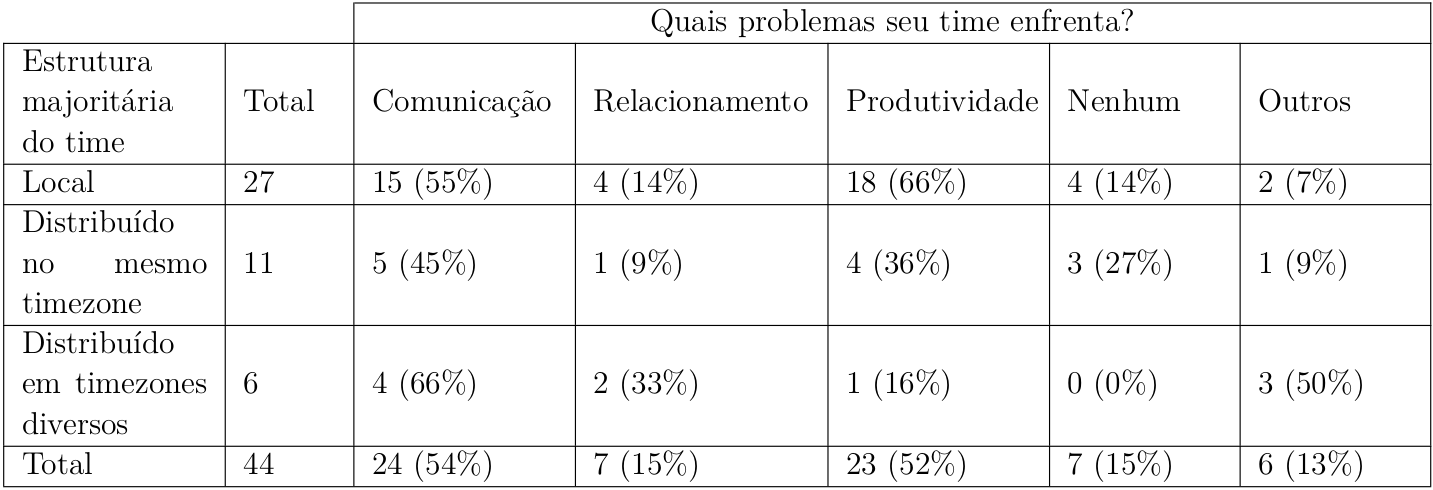
\includegraphics[width=0.8\textwidth]{problemasTime.png}
\caption{Problemas enfrentados pelos times}
\label{tab:problemasTime}
\end{table}

O desafio mais enfrentado por times ágeis em geral é a comunicação e a estrutura que apresentou maiores dificuldades com isto foram os times distribuídos em \textit{timezones} diversos. Outro desafio que estes times aparentam ter mais dificuldades do que os locais e distribuídos no mesmo fuso horário é o relacionamento. Além disso, os times distribuídos em \textit{timezones} diversos foram os que mais apresentaram ''Outros'' problemas. Uma dificuldade apontada que chama a atenção foi de sincronizar seus membros.

Apesar dessa distribuição ter mais problemas de comunicação, relacionamento e outros, eses times possuem o melhor rendimento. Apenas 16\% apresentaram problemas de produtividade, enquanto os distribuídos no mesmo \textit{timezone} chegaram a 36\% e os locais em 66\%.

Depois de encontrar os desafios enfrentados por cada um dos times ágeis, os próximos resultados demonstram como a melhoria contínua é promovida.

\begin{table}[ht]
\centering
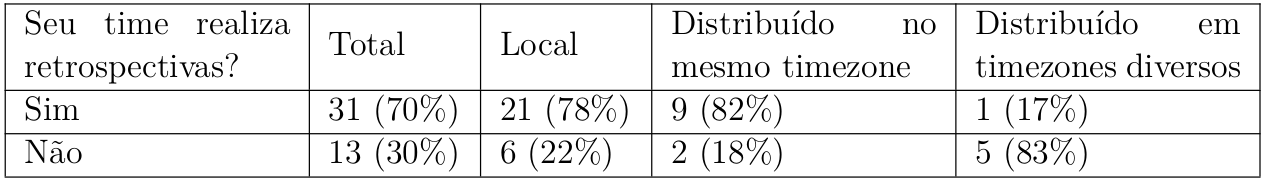
\includegraphics[width=0.45\textwidth]{retrospectiva.png}
\caption{Uso da retrospectiva}
\label{tab:retrospectiva}
\end{table}

Os resultados na Table~\ref{tab:retrospectiva} foram próximos dos obtidos pela State of Agile Report \cite{version:15} e State of Scrum Report \cite{scrum:15}, dado que aproximadamente 70\% dos participantes realizam retrospectivas. No entanto, é importante notar que apenas 16\% dos distribuídos em \textit{timezones} diversos realizam retrospectivas, mostrando que ela não é uma unanimidade para todos os formatos das equipes.

Uma questão que também é pouco abordada pelas pesquisas e artigos na comunidade é se a retrospectiva realmente auxilia os times a resolver seus problemas. Para investigar esta questão, é possível fazer uma relação entre os problemas apontados e o fato do time realizar ou não a retrospectiva.

\begin{table}[ht]
\centering
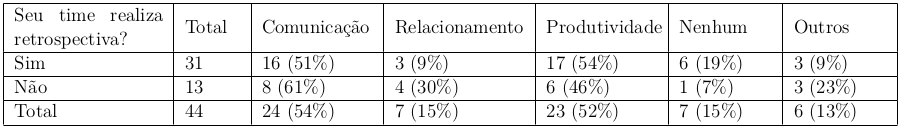
\includegraphics[width=0.8\textwidth]{retrospectivaValeAPena.png}
\caption{Relação entre retrospectiva e os problemas dos times ágeis}
\label{tab:retrospectivaValeAPena}
\end{table}

Os resultados na Table~\ref{tab:retrospectivaValeAPena} mostram que a retrospectiva ajuda os times ágeis para os problemas de comunicação, relacionamento e outros. O único resultado contrário foi a produtividade, dado que os times que não realizam retrospectivas apresentaram melhores resultados neste quesito com um percentual de 46\%. Um hipótese para estes números é por conta da maior parte dos times que responderam ''Não'' serem da categoria times distribuídos em timezones diversos. Como apresentado anteriormente, eles mostraram os melhores resultados em termos de produtividade, o que pode ter influenciado o resultado.

Outro fator a se notar é a quantidade de respostas na opção  ''Nenhum''. Apenas 7\% dos times que não usam a retrospectiva assinalaram esta opção, enquanto para os que a realizam foram 19\%. Apesar de parecer um ponto positivo não ter nenhuma dificuldade, é suspeito não ter nem mesmo um único problema. Pode ser um indicativo de que estes são os times com os maiores problemas, já que é mais provável que eles existam, mas as pessoas não estão cientes deles.

A pesquisa mostrou que retrospectiva têm de fato auxiliado os times no processo de melhoria contínua. No entanto, é notável que ainda há espaço para esta reunião melhorar e ajudar ainda mais as equipes. Desta forma, os próximos resultados mostram em quais pontos os times enfrentam mais dificuldades durante a reunião.

\begin{table}[ht]
\centering
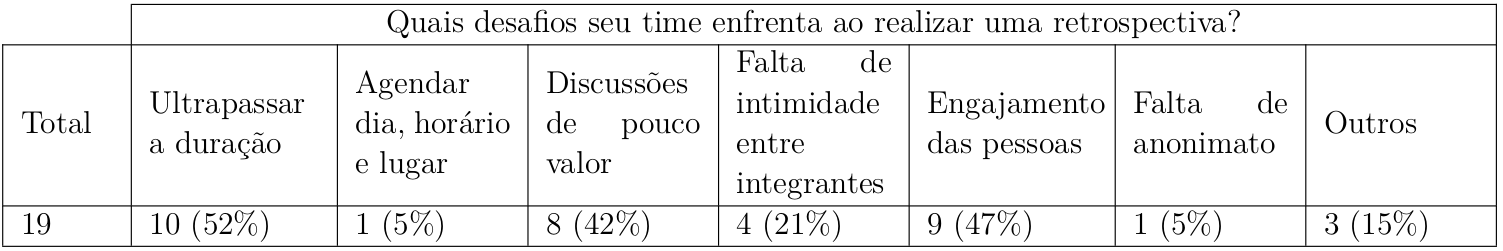
\includegraphics[width=0.8\textwidth]{problemasRetrospectiva.png}
\caption{Desafios da retrospectiva}
\label{tab:problemasRetrospectiva}
\end{table}

Segundo a Table~\ref{tab:problemasRetrospectiva}, os principais desafios enfrentados são ultrapassar a duração, falta de engajamento das pessoas e discussões de pouco valor. Uma hipótese defendida por Poussard \cite{poussaard:14} é que quando se repete o mesmo formato de retrospectiva, geralmente é uma das causas para haver a falta de engajamento dos integrantes e as discussões tem um menor valor.

\begin{table}[ht]
\centering
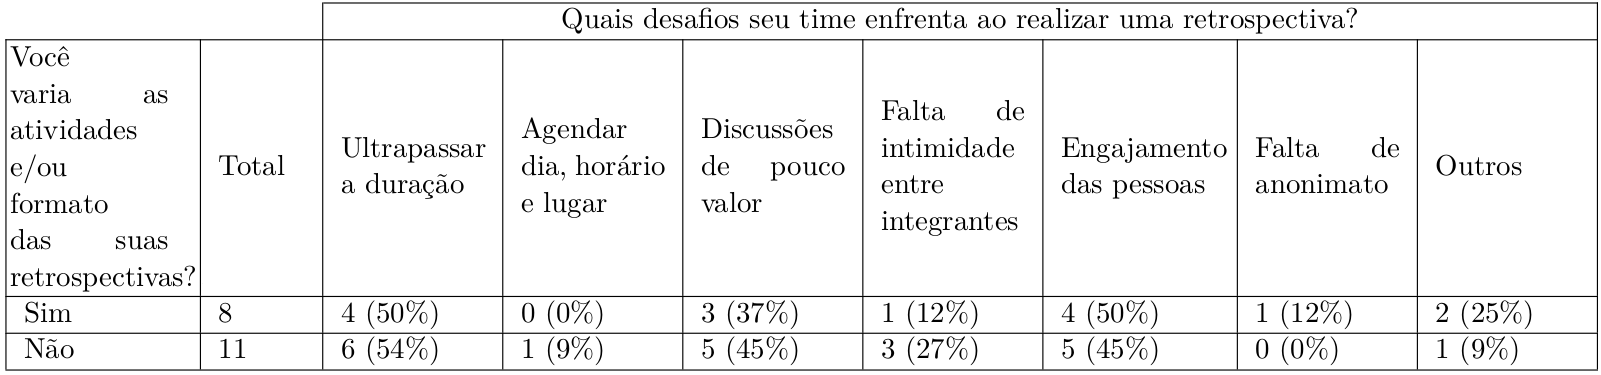
\includegraphics[width=1\textwidth]{variarRetrospectiva.png}
\caption{Times que variam a retrospectiva}
\label{tab:variarRetrospectiva}
\end{table}

A Table~\ref{tab:variarRetrospectiva} mostrou a relação que existe entre os desafios e variar ou não as atividades. Alguns dos números confirmaram as hipóteses de Poussard, como as equipes que não variam as retrospectivas terem mais discussões de pouco valor. Além disso, os times que variam suas atividades aparentam sofrer menos com falta de intimidade entre integrantes. No entanto, para a falta de engajamento das pessoas os números foram parecidos e os times que responderam ''Não'' tiveram um percentual um pouco melhor, contrariando as expectativas. Então apenas variar as atividades não é suficiente para enfrentar os desafios dessa reunião.

\subsection{Resultados das perguntas qualitativas}

Já as questões qualitativas focaram principalmente para os times que não fazem retrospectiva. Uma das perguntas questionava quais os motivos levaram a equipe não usar a retrospectiva, para investigar o porquê do baixo número de equipes geograficamente distribuídas fazendo retrospectiva. A hipótese inicial era que estes times não faziam a reunião devido à impossibilidade de reunir todos os membros para uma discussão em algum horário.

Duas respostas mostraram que uma razão para o time não realizar a retrospectiva é devido a falta de tempo, já que ambos alegaram que a equipe está passando por período de alta demanda. Outros dois participantes responderam que o motivo vem a partir de uma decisão dos gestores do projeto. E uma destas respostas também revelou que o gerente não possui experiência com metodologias ágeis. O último participante também indicou que não é cultura da empresa utilizar desta prática. 

Com apenas estas informações não é possível tirar conclusões definitivas sobre o porquê deles não realizarem retrospectivas. Uma hipótese é que esses times ainda não possuem experiência suficiente com métodos ágeis e também não dispõem de pessoas engajadas em agilidade que queiram aplicar retrospectivas como forma de inspecionar problemas. Logo, eles acabam não vendo o valor da reunião e o retorno que ela proporciona. Essa hipótese é reforçada a partir das respostas sobre como os problemas nesses times são discutidos e resolvidos.

Os times que responderam anteriormente que não fazem retrospectivas devido a alta demanda indicaram que realizam conference calls para debater sobre os problemas do time. Em geral, essas reuniões não tem um horário previsto para acontecer e todos os integrantes participam. Neste ponto existe uma inconsistência entre as respostas, pois ambos alegam que o time não possui tempo para realizar a retrospectiva, mas eles conseguem mobilizar as pessoas para uma reunião onde são discutidos os problemas. Da mesma forma, também houve inconsistências nas respostas dos outros times que apontaram que a decisão foi dos gestores ou por não ser cultura da empresa. Estes times conversam via chat para discutir os seus problemas e os membros que possuem disponibilidade participam ativamente do debate. Caso as pessoas encontrem uma solução interessante, ela é informada para o restante da equipe e gerente do projeto.

Como nenhum dos participantes mencionou o nome da prática de melhoria contínua usada, não é possível concluir se estas reuniões são baseadas em algum outro tipo de prática ágil conhecida. No entanto, nota-se que este formato é muito semelhante à retrospectiva. Provavelmente a única diferença é que algumas das atividades utilizadas em retrospectivas motivam o time a conversar sobre o futuro. Quando questionados de que forma o time identifica os problemas futuros e trabalha para evitá-los, a grande maioria indicou que não possuem esse tipo de preocupação. Apenas um participante comentou que existe essa discussão, mas focada apenas no código da aplicação.

\section{Próximos passos}

Devido ao número de respostas, parte dos resultados não foram conclusivos e alguns deles contrariam hipóteses apresentadas por outros artigos. Além disso, não foi possível descobrir exatamente como os times que não utilizam retrospectiva estão promovendo a melhoria contínua, principalmente os distribuídos.

O próximo passo é desenvolver uma nova pesquisa direcionando as perguntas para encontrar as respostas para estas dúvidas. Outro objetivo para a próxima pesquisa é atingir um maior número de times para ter uma base mais consistente e diversificada. A maior parte dos times não distribuídos que responderam a pesquisa se localizavam no Brasil, então seria interessante conseguirmos descobrir como funcionam os times ágeis em outros países.

\section{Conclusão}

No início deste estudo, era visível uma carência de informações sobre como times promovem melhoria contínua. A partir desta pesquisa, obteve-se algumas informações interessantes sobre este assunto, como o fato de que a maioria dos times locais ou que trabalham no mesmo fuso ainda usam a retrospectiva. E esta reunião de fato os ajuda a resolver boa parte dos seus problemas, como comunicação, relacionamento, entre outros. No entanto, a partir do momento que os integrantes estão se espalhando ao redor do mundo, esta reunião começou a deixar de ser uma tendência no mercado.

Nota-se que muitos destes times distribuídos em diversos fuso horários que não fazem retrospectiva estão usando modelos parecidos de discutir o que está funcionando e o que pode ser melhorado, só que de uma forma mais assíncrona. Mesmo assim, ainda não é possível garantir que esta seja a única forma que existe atualmente com a baixa quantidade de dados obtidas para estas equipes.

Mesmo assim, é possível perceber que o processo de melhoria contínua para as estruturas mais conhecidas, como de times locais e distribuídos no mesmo fuso horário, está mais adaptado devido ao tempo que a reunião já vem sendo utilizada por estes times. No entanto, para os times distribuídos em diversos timezones, que viraram tendência no mercado nos últimos 5 anos, parece que este princípio ainda vem passando por processos de adaptação e não existe uma forma clara de como agir nestes contextos. É necessário uma investigação mais a fundo especificamente nesta área para encontrar os padrões entre as práticas que estas equipes vem adotando.

\bibliographystyle{sbc}
\bibliography{sbc-template}

\end{document}
